\chapter{Introduction}
\label{chapter1}

\section{Background and Motivation}
The Sun, an ordinary main-sequence star situated at the center of our solar system, exhibits various forms of activity and variability on multiple spatial and temporal scales. Some of the main manifestations of solar activity relevant to space weather research (Fig.~\ref{fig_sw}) are transient energetic eruptive phenomena such as solar flares, Coronal Mass Ejections (CME), and wide-ranging emissions of electromagnetic radiation and energetic particles \citep{schwenn_2006, pulkkinen_2007}. These eruptive events originate due to the sudden release of free magnetic energy stored in complex, twisted or sheared magnetic field structures in the solar atmosphere \citep{moore_2001, priest_forbes_2007, zhang_2012, amari_2014}. The energetic phenomena are driven by the rapid dissipation of magnetic energy via magnetic reconnection which can accelerate large numbers of electrons to relativistic energies and heat plasma to tens of million Kelvin \citep{shibata_2011, benz_2017}.

The eruptive solar events drive major disturbances in the near-Earth space environment and planetary environments across the heliosphere, collectively termed \textit{space weather} \citep{schrijver_2010, eastwood_2017}. Enhanced fluxes of Solar Energetic Particles (SEPs), plasma ejecta, and electromagnetic radiation emitted during solar eruptions can impact the geomagnetic field, radiation belts, ionosphere, thermosphere, and upper atmosphere surrounding the Earth \citep{schwenn_2006, pulkkinen_2007}. Adverse effects range from disruption of radio communications to damage of satellites, power grid failures, aviation hazards due to radiation risks for airline crew and passengers, and increased radiation exposure for astronauts \citep{lanzerotti_2001}. The societal dependence on space-based infrastructure has increased exponentially, escalating the vulnerability to space weather disturbances. Recent studies estimate a severe space weather event could lead to trillion-dollar economic damages in the US alone \citep{oughton_2017}. Besides the near-Earth space environment, solar eruptive transients also drive adverse space weather effects across the solar system impacting activities such as deep space exploration and astronomy \citep{lilensten_2014}.

Therefore, advancing our understanding of the origins and propagation characteristics of solar eruptive phenomena, as well as quantifying their impacts on geospace and planetary environments, has become an extremely important pursuit for nations worldwide. Fundamental research seeks to uncover the physical processes involved using observations coupled with theory and modeling. Concurrently, significant efforts are underway to develop next-generation space environment modeling and forecasting capabilities for predicting the impacts of solar variability. The field combining these research and predictive aspects related to Sun-Earth connections is broadly termed \textit{heliophysics} \citep{schrijver_siscoe_2010}. It encompasses understanding the fundamental solar, heliospheric and geospace plasma processes; coupling across multiple spatial and temporal scales; quantifying the impacts on humanity's technological systems and space-borne assets; and utilizing this knowledge to prevent or mitigate adverse effects \citep{schrijver_2015a, schrijver_2015b}. NASA's Living With a Star program and the National Science Foundation's Space Weather activities exemplify strategic efforts to advance scientific understanding and predictive capabilities across the interconnected domains of heliophysics \citep{brewer_2002}.

The present thesis focuses on studying several important phenomena related to solar eruptive activity and its impacts from the perspective of heliophysics research and space weather. The specific topics investigated include: (1) the propagation and evolution characteristics of large-scale coronal disturbances termed Extreme Ultra-Violet (EUV) waves that are triggered by CMEs and solar flares; (2) the generation, propagation and plasma characteristics of solar radio bursts emitted by accelerated electron beams traveling along open magnetic field lines in the corona; (3) the forecasting of SEP events which constitute one of the major components of space radiation hazards at Earth.

\begin{figure}[!htp]
	\centerline{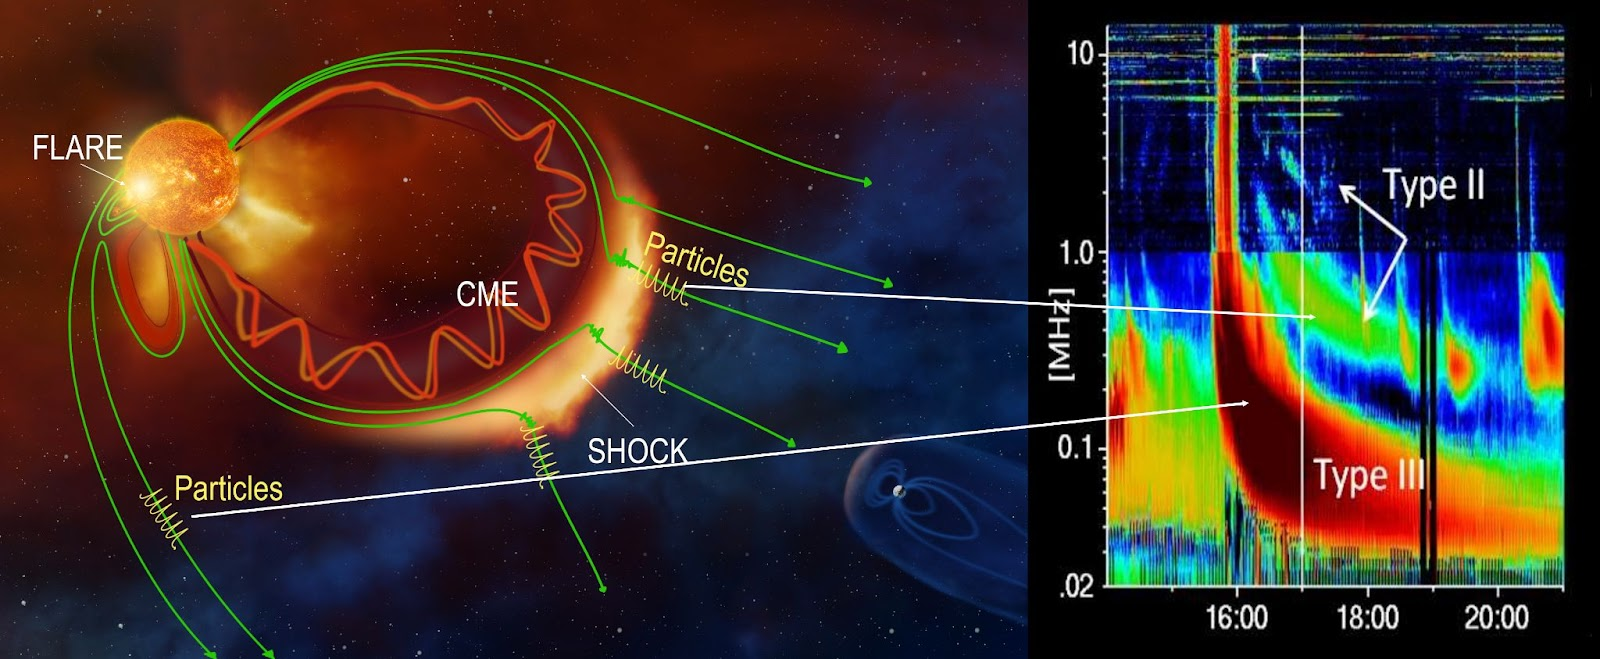
\includegraphics[width=0.9\columnwidth]{chapter1/figs/srbs.jpeg}}
	\caption{On the left side, a graphical illustration, adapted from ESA/A. Baker, CC BY-SA 3.0 IGO, depicts different eruptive phenomena, while on the right side, there is a representation of spacecraft data (specifically Wind/Waves data from \citet{gopalswamy_2019}) showcasing a radio dynamic spectra, emphasizing distinct spectral categories of SRBs on November 9, 2000. Type-II bursts are correlated with the shock front of a CME, whereas Type-IIIs are connected with the acceleration of SEPs. Image courtesy\protect\footnotemark}
	\label{fig_sw}
\end{figure}

These diverse topics are united by the common theme of seeking to uncover the origins and propagation mechanisms of key transient phenomena resulting from solar eruptions, utilizing observational data, analytical theory and modeling, and data science techniques. The phenomena have been studied for several decades using observations from multiple space missions, but gaps persist in our understanding of their underlying physics and space weather impacts. The thesis aims to provide new insights that help address some of the outstanding questions, guided by the overarching goals and framework of heliophysics research. Each research topic investigated in this thesis is explored in detail within its dedicated chapter. These chapters delve into the relevant background, significance, observational challenges, and knowledge gaps associated with each topic. Additionally, a concise overview of key literature related to each topic is provided here, followed by a more in-depth review within each specific chapter.

\footnotetext{\url{https://www.dias.ie/cosmicphysics/astrophysics/astro-surround/}}

\subsection{Coronal Waves}
Coronal waves, or Coronal Bright Fronts (CBFs), also known as EUV waves, are large-scale arc-shaped bright fronts or disturbances observed propagating across significant portions of the solar corona following the eruption of CMEs and solar flares \citep{thompson_1998, nindos_2008, vrsnak_2008, magdalenic_2010, veronig_2010, warmuth_2015}. They are best observed in EUV and white-light coronal emission, as well as in radio wavelengths, spanning distances of up to several 100 Mm with speeds ranging between 100-1000 \kms, faster than the local characteristic speed in the solar corona, transforming into shock waves \citep{pick_2006, thompson_2009, nitta_2013, liu_2014}. These structures consist of piled-up plasma with higher density, making them appear brighter in white-light images.

The discovery of coronal waves dates back to observations obtained with the Extreme ultraviolet Imaging Telescope (EIT) instrument on the Solar and Heliospheric Observatory (SOHO) launched in 1995, appearing as bright propagating fronts in 19.5 nm wavelength imaging of Fe XII emission lines formed at \almost1.5 MK plasma \citep{thompson_1998}. Subsequent studies based on SOHO/EIT and the Transition Region and Coronal Explorer (TRACE) imaging found correlations between coronal waves and CMEs, favoring an interpretation as fast-mode magneto-hydrodynamic (MHD) waves driven by CME lateral expansions \citep{biesecker_2002}.

Since 2010, the initiation and evolution of coronal waves are being exquisitely observed with unprecedented resolution by the Atmospheric Imaging Assembly (AIA) on the Solar Dynamics Observatory (SDO) spacecraft \citep{lemen_2012} across multiple EUV passbands sensitive to a wide temperature range \citep{nitta_2013}.
Observing and studying coronal shock waves remotely is typically done through EUV observations using space-based instruments such as the AIA onboard the SDO spacecraft. Alternatively, shock waves can be indirectly observed through the detection of type II radio bursts, which are commonly associated with shock waves in the solar corona \citep{vrsnak_2008}.
%Alternatively, shock waves can be indirectly observed through the detection of type II radio bursts, which are commonly associated with shock waves in the solar corona \cite{vrsnak_2008}.

The AIA instrument has provided valuable insights into the dynamics of the low solar corona over the past decade, thanks to its exceptional spatial and temporal resolution. Equipped with telescopes observing the solar disk in bands 193 and 211~\AA, the AIA instrument has demonstrated its ability to distinguish compressive waves in the lower corona \citep{patsourakos_2010, ma_2011, kozarev_2011}. These observations offer valuable information about the kinematics and geometric structure of CBFs. To accurately study the evolution of the wave's leading front, observations off the solar limb are preferred to mitigate projection effects, which may introduce ambiguities in estimating time-dependent positions and the global structure of the wave \citep{kozarev_2015}.
Figure~\ref{fig_cme} shows a CME launched form the east limb on June 13, 2022, depicting the typical three-part structure of CMEs. The image of the solar disk at the center of the figure is obtained from the SDO/AIA instrument at 04:12:05 UT, while the outer coronagraph image is obtained from the SOHO/LASCO instrument at 04:12:07 UT. The SOHO/EIT imaging data was not available at that time.

Typically, CMEs have three parts \citep{vourlidas_2013}:
\begin{itemize}
	\item \textbf{CME Front}: This refers to the leading edge of a Coronal Mass Ejection (CME), which can take on various shapes, such as loop-like or halo-shaped, depending on its position relative to the Sun's limb. The bright loop often observed represents plasma accumulation at the boundary of the erupting flux rope, while the faint front preceding it is caused by density compression at a wave or shock front propelled by the CME.
	
	\item \textbf{CME Cavity}: This is a zone characterized by reduced density and magnetic field strength located behind the CME front. It forms as the prominence material, cool and dense, settles along the dips of the magnetic field lines that compose the flux rope. Initially, during the eruption's early stages, most of the prominence material either moves towards the solar surface or heats up to coronal temperatures. In coronagraphic imagery, the CME cavity appears as a dark area enclosed by the bright CME front.
	
	\item \textbf{CME Core}: This central region of the CME encompasses the erupting plasma, where the magnetic field lines are heavily twisted and carry significant magnetic energy.
\end{itemize}
%The AIA instrument has provided valuable insights into the dynamics of the low solar corona over the past decade, thanks to its exceptional spatial and temporal resolution. Equipped with telescopes observing the solar disk in bands 193 and 211 $\AA$, the AIA instrument has demonstrated its ability to distinguish compressive waves in the lower corona \cite{patsourakos_2010, ma_2011, kozarev_2011}. These observations offer valuable information about the kinematics and geometric structure of CBFs. To accurately study the evolution of the wave's leading front, observations off the solar limb are preferred to mitigate projection effects, which may introduce ambiguities in estimating time-dependent positions and the global structure of the wave \cite{kozarev_2015}.
\begin{figure}[!htp]
	\centerline{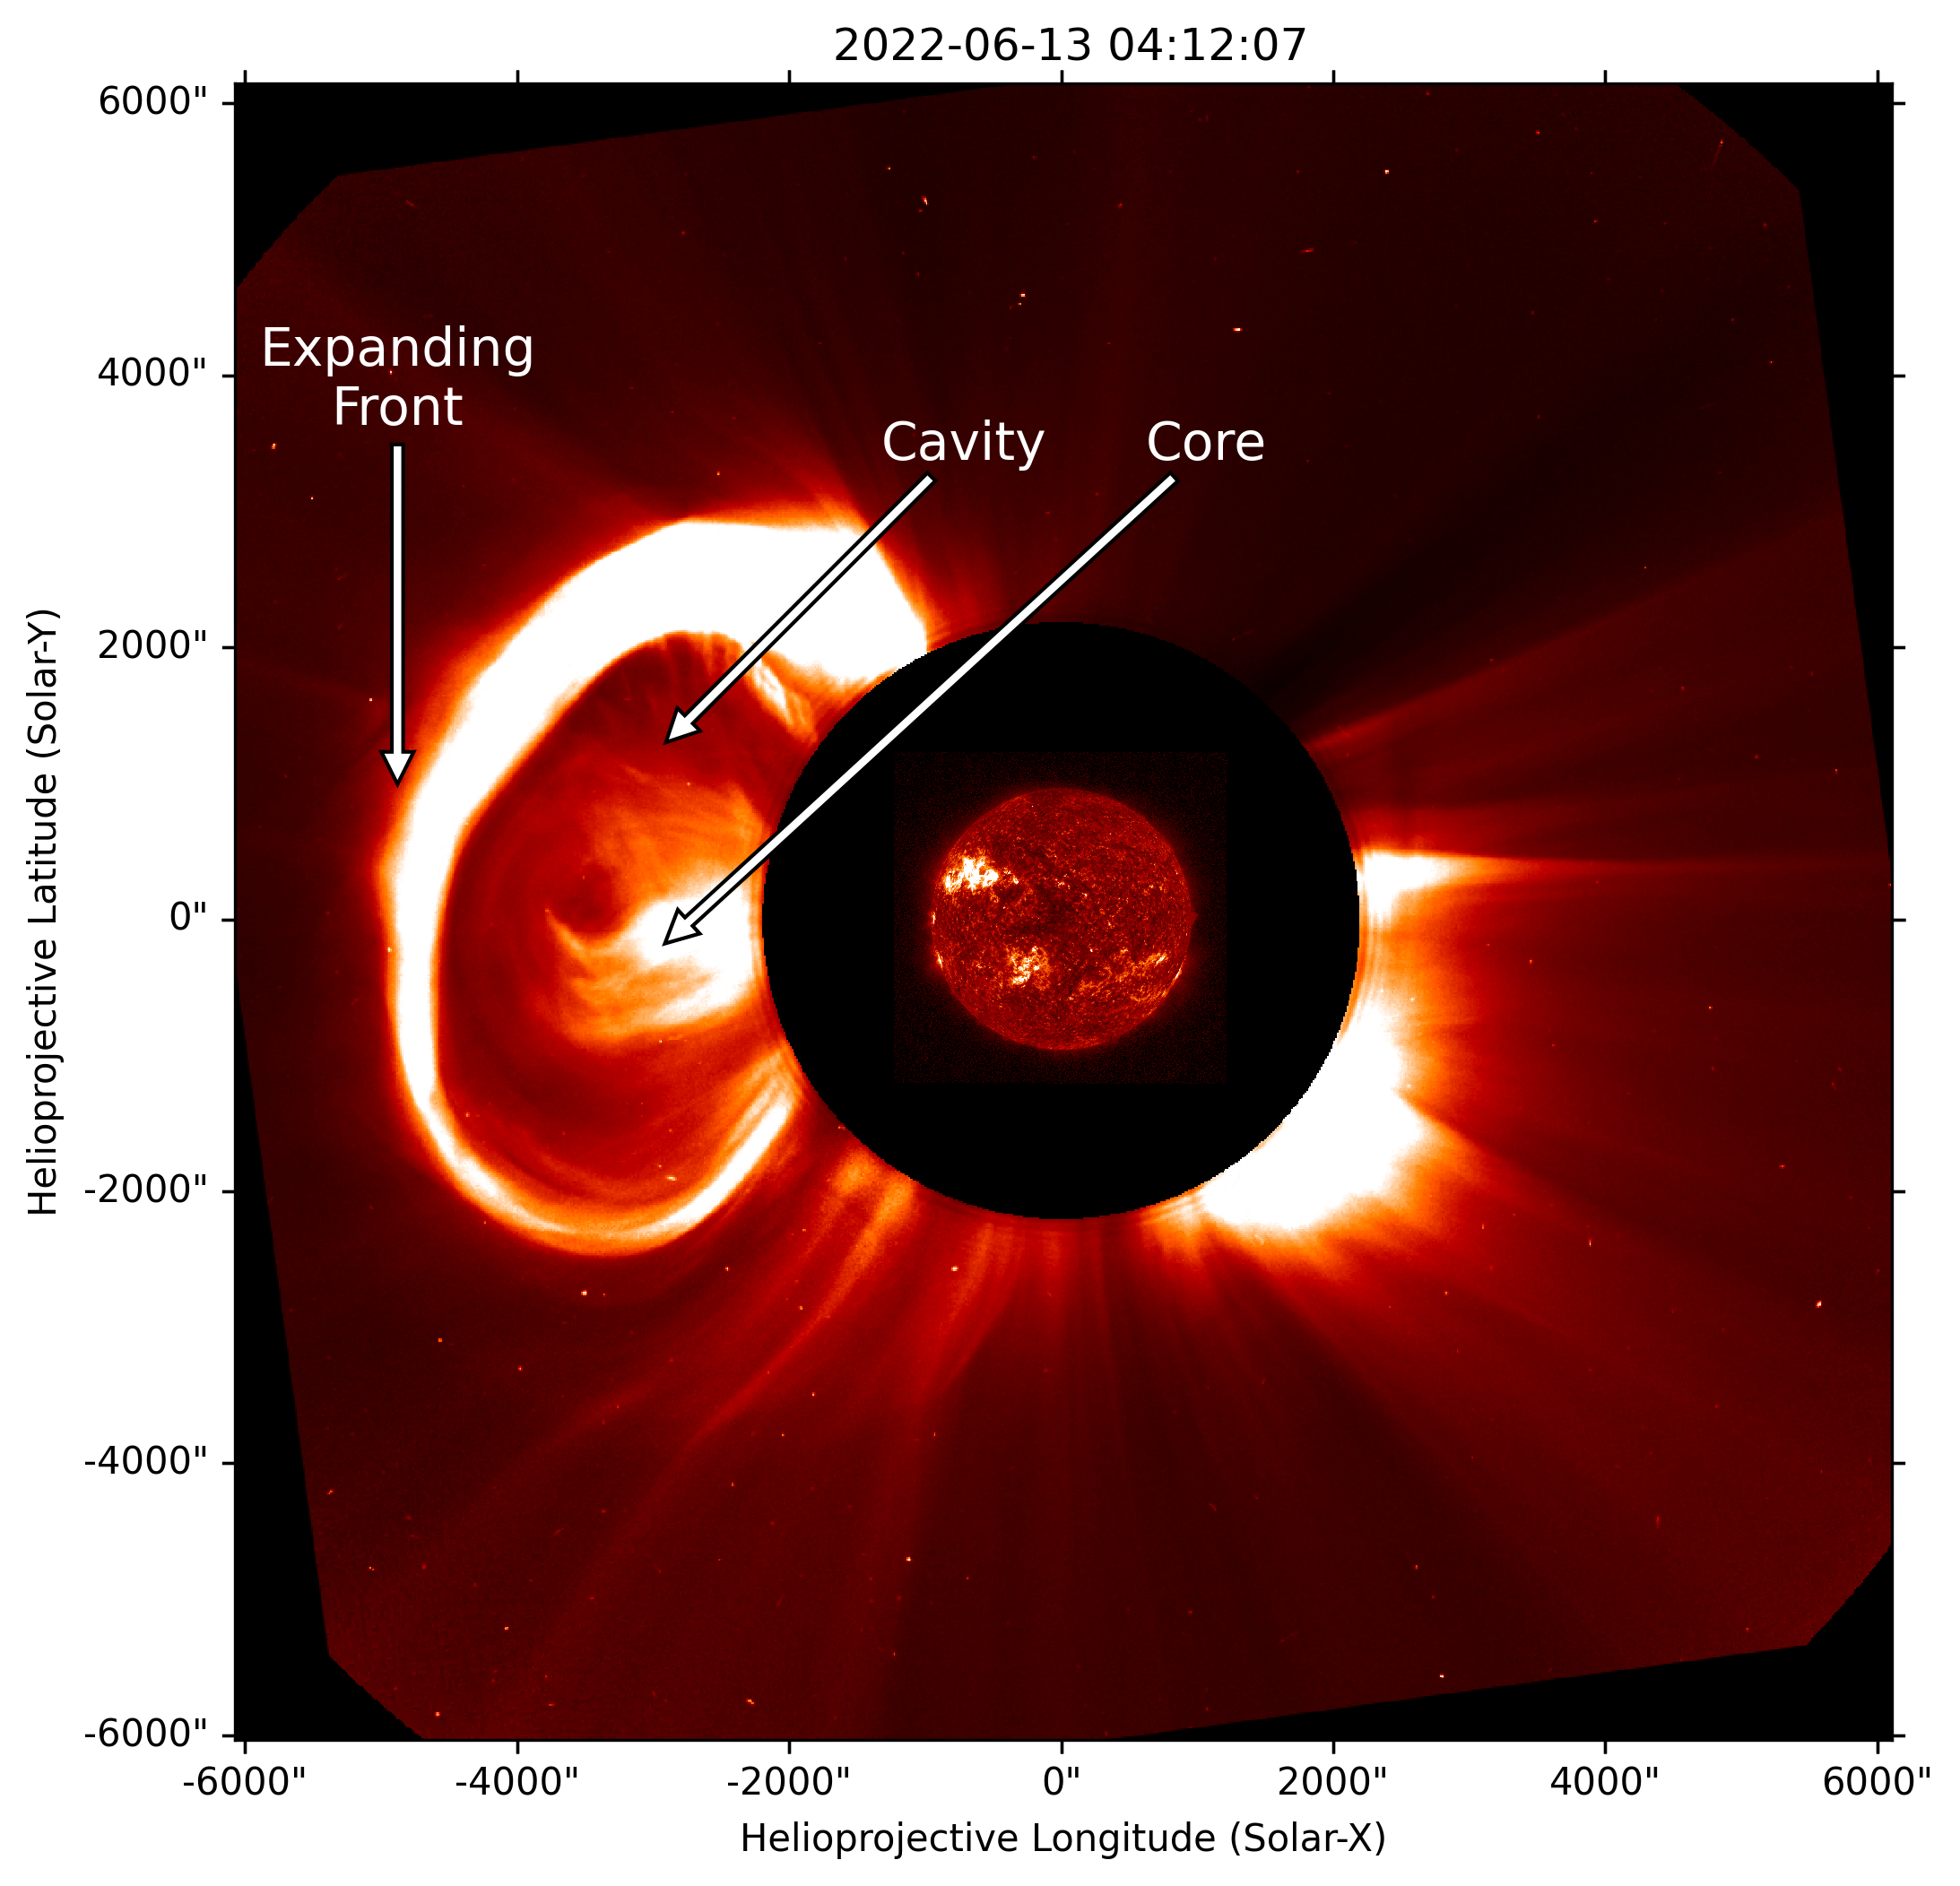
\includegraphics[width=0.8\columnwidth]{chapter1/figs/AIA_LASCO_composite_2022613.png}}
	\caption{Composite image from the AIA and LASCO telescopes on the NASA-GSFC SDO and NASA/ESA SOHO spacecrafts shows a large CME being ejected to the east and its typical structure.}
	\label{fig_cme}
\end{figure}

CBFs are formed in front of the expanding front of CMEs. In situ observations of shock waves have revealed their classification into quasi-parallel, quasi-perpendicular, sub-critical, and super-critical shocks based on the angle between the wavefront normal vector and the upstream magnetic field lines \citep{tsurutani_1985}. Quasi-parallel shocks have a shock-field angle ($\theta_{BN}$) smaller than 45\degree, while quasi-perpendicular shocks have $\theta_{BN}$ greater than 45\degree. Supercritical shocks, often associated with accelerated particles, are promising candidates for generating type II radio bursts \citep{benz_1988}. However, obtaining accurate estimates of shock strength and obliquity solely from remote observations is challenging.
%In situ observations of shock waves have revealed their classification into quasi-parallel, quasi-perpendicular, sub-critical, and super-critical shocks based on the angle between the wavefront normal vector and the upstream magnetic field lines \cite{tsurutani_1985}. Quasi-parallel shocks have a shock-field angle ($\theta_{BN}$) smaller than 45\degree, while quasi-perpendicular shocks have $\theta_{BN}$ greater than 45\degree. Supercritical shocks, often associated with accelerated particles, are promising candidates for generating type II radio bursts \cite{benz_1988}. However, obtaining accurate estimates of shock strength and obliquity solely from remote observations is challenging.

Coronal waves exhibit diverse morphology and kinematics ranging from circular fronts to narrow jets or expanding dome-like structures \citep{veronig_2010}. A taxonomy of wave properties based on extensive observational surveys can be found in papers by \citet{muhr_2014} and \citet{nitta_2013}. However, despite being observed for over two decades since their serendipitous discovery, fundamental questions remain regarding the physical nature and drivers of coronal waves \citep{chen_2016, vrsnak_2008, warmuth_2015}. The debate centers around two competing interpretations -- the wave versus pseudo-wave (or non-wave) models. The wave models envisage coronal waves as fast-mode MHD waves or shocks that propagate freely after being launched by a CME lateral over-expansion or an initial flare pressure pulse \citep{wills_2007, vrsnak_2008}. The pseudo-wave models interpret them as bright fronts produced by magnetic field restructuring related to the CME lift-off process rather than a true wave disturbance \citep{delannee_1999, chen_2002}.

Extensive observational and modeling studies have been undertaken to evaluate the two paradigms \citep{patsourakos_2012, long_2017}, but a consensus remains elusive. Addressing these outstanding questions related to the nature and origin of coronal waves is imperative, since they are being incorporated into models as a primary agent producing SEP events and geomagnetic storms following CMEs \citep{rouillard_2012, park_2013}. Their use as a diagnostic tool for CME and shock kinematics predictions in these models requires discriminating between the different physical mechanisms proposed for their origin.

The present thesis undertakes an extensive statistical analysis of coronal EUV wave events observed by SDO to provide new insights into their kinematical properties and relationship to CMEs. I focus on analyzing their large-scale evolution as a function of distance and direction from the source region, leveraging the extensive EUV full-disk imaging capabilities of SDO spanning nearly a decade. Statistical surveys to date have mostly focused on initial speeds and morphological classifications rather than large-scale propagation characteristics. The first study presented in Chapter~\ref{chapter2} aims to uncover systematic trends in their propagation kinematics using a combination of techniques and data products, as well as exploring relationships between different pairs of kinematical parameters compared to previous works.
%We also comprehensively evaluate associations with CME and plasma parameters in order to discriminate between wave and pseudo-wave origins.
The results have important implications for incorporating coronal waves into predictive models of CMEs and SEP events for future space weather forecasting.

\subsection{Solar Radio Bursts}
Solar radio emissions have been the subject of extensive study and research due to their connection with solar activity and their potential impact on Earth's atmosphere and technology. One area of particular interest is solar radio bursts, which are intense bursts of electromagnetic radiation originating from the Sun. These bursts can be classified into different types based on their characteristics and associated phenomena. Solar radio bursts, including type III bursts, serve as remote diagnostics for the study of energetic electrons within the solar corona. These bursts result from transient energetic electron beams injected into the corona, which then propagate along interplanetary magnetic field (IMF) lines \citep{ergun_1998, pick_2006, reid_2020}. As these electron beams traverse the corona, they induce plasma waves, also known as \textit{Langmuir waves}, which subsequently transform into radio emission at the local plasma frequency or its harmonic components \citep{melrose_2017}.
The frequency of the radio emission is directly linked to the plasma density, making type III bursts a valuable tool for investigating the inner heliosphere and understanding the underlying processes that drive solar active phenomena, such as CMEs and solar flares \citep{reid_2014, kontar_2017}. These bursts offer insights into the acceleration of energetic electrons in the corona and their transport along magnetic field lines \citep{reid_2014}. The generation of electromagnetic emission at radio frequencies through plasma emission mechanisms is a key aspect of solar radio bursts, shedding light on the dynamic interplay between non-thermal electron distributions and the ambient plasma \citep{melrose_1980}.

Pioneering observations of solar radio bursts were made in the 1940s leading to their classifications \citep{wild_1963}. Subsequent spectrographic studies uncovered emission mechanisms, source regions and particle diagnostics \citep{suzuki_1985}. Magnetic reconnection models of flares provided theoretical explanations for particle acceleration generating radio bursts \citep{holman_2011}. Radio imaging spectroscopy using interferometric imaging arrays coupled with high time-frequency resolution spectrometers enables tracking radio sources as a function of frequency and position on the Sun, yielding particle acceleration locations and trajectories through the corona into interplanetary space \citep{krucker_2011, klassen_2003a, klassen_2003b}. This provides a unique diagnostic of energetic particle transport from the Sun to the Earth which is crucial for improving SEP forecasting models.

Different types of bursts are observed (Fig.~\ref{fig_srb_types}), classified based on their spectral characteristics as documented in radio burst catalogs \citep{wild_1963}. The present thesis focuses on detailed analysis of solar type III radio bursts and their associated phenomena.
In radio spectrograms, type III radio bursts manifest as intense enhancements of radio flux exceeding background levels. These bursts exhibit rapid frequency drifts over timescales ranging from seconds to minutes, reflecting the underlying plasma dynamics \citep{reid_2017}. Notably, they are observable across a broad spectrum of frequencies, spanning from GHz to kHz, and corresponding wavelengths extending from metric to decametric \citep{wild_1950a, lecacheux_1989, bonnin_2008}. This phenomenon is detectable by ground-based instruments on Earth as well as various spacecraft within the heliosphere, underscoring the significance of plasma dynamics in their manifestation.

\begin{figure}[!htp]
	\centering
	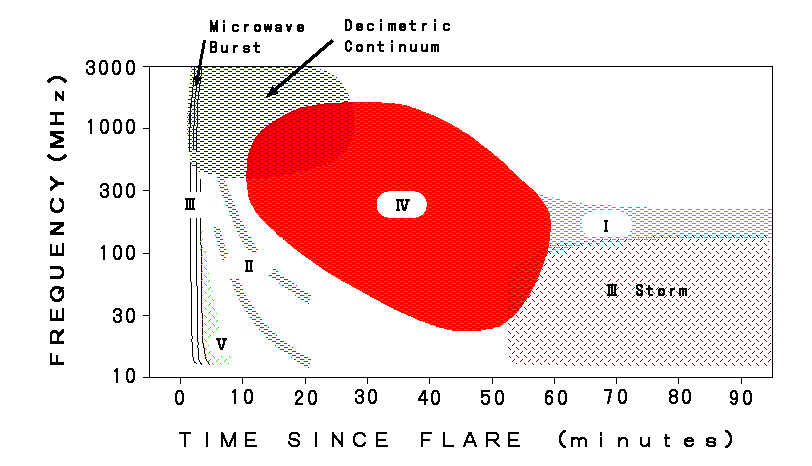
\includegraphics[width=0.8\columnwidth]{chapter1/figs/typefignew.png}
%	\caption[Classification of solar radio bursts]{Diagram illustrating the classification of solar radio bursts. Image courtesy\footnote{Types of solar radio bursts: \url{http://solar.physics.montana.edu/takeda/radio_burst/srb.html}}.}
	\caption[Classification of solar radio bursts]{Diagram illustrating the classification of solar radio bursts. Image courtesy\protect\footnotemark}
	\label{fig_srb_types}
\end{figure}

Furthermore, these bursts arise from the propagation of energetic electron beams ejected during magnetic reconnection. The observed rapid drift from high to low frequencies over seconds directly corresponds to the propagation of these electron beams from the Sun's lower corona, outward along open magnetic field lines, potentially extending beyond 1 astronomical unit (AU). This characteristic signature signifies the initial escape of flare-accelerated electrons into interplanetary space, making type III bursts a crucial precursor for subsequent SEP activity \citep{cane_2002, macdowall_2003}.
Investigating their source locations, plasma environments, and beam kinematics based on multi-wavelength observations coupled with plasma emission theory is therefore vital for improved understanding of coronal particle acceleration and transport processes relevant for SEP forecasting models.

While type III bursts have been studied for over 50 years since their initial discovery by \citet{wild_1950a, wild_1950b, wild_1950c}, gaps persist in our understanding of their exciter beams and emission mechanisms. Key outstanding questions pertain to the detailed electron acceleration and injection sites, beam configurations and energy spectra, drivers of burst onset and duration, and the role of density fluctuations in propagating beams \citep{reid_2018a, reid_2018b, li_2012a}. Recent work combines imaging and spectral data with modeling to constrain radio burst exciters in unprecedented detail \citep{chen_2013b, kontar_2017}. Key challenges remain in reconciling emission models with observations and predicting radio diagnostics. Advancing our knowledge of these aspects through coordinated observations and modeling can help constrain the predictions of energetic electron properties based on radio diagnostics. The present work undertakes detailed investigation of a solar type III burst combining imaging and radio spectral data to derive electron beam trajectories and coronal densities, and models the emission sources. The results provide insights into the corona plasma environment and energetic electron transport relevant for SEP forecasting applications.

\footnotetext{Types of solar radio bursts: \url{http://solar.physics.montana.edu/takeda/radio_burst/srb.html}}

\subsection{Solar Energetic Protons Forecasting}
Solar energetic protons are high-energy particles that are believed to originate from the acceleration of particles in the solar corona during solar flares and CMEs \citep{aschwanden_2002, lin_2005, lin_2011, klein_2017, kahler_2017}. They are typically characterized by their high energy levels -- with some particles having energies in the relativistic GeV/nucleon range -- and their ability to penetrate through spacecraft shielding, causing radiation damage \citep{reames_2013, desai_2016}. The fluence and energy spectrum of SEP are influenced by several factors, including the strength of the solar flare or CME that produced them, and the conditions of the interplanetary environment \citep{kahler_1984, kahler_1987, debrunner_1988, miteva_2013, trottet_2015, dierckxsens_2015, le_2017, gopalswamy_2017}. In this thesis, I will refer to solar energetic protons as SEPs since they are the major constituents of solar energetic particle events.

SEP exhibit a strong association with the solar cycle, with the frequency and flux of SEP events peaking during the maximum phase of the solar cycle \citep{reames_2013}. This is thought to be due to the increased activity of the Sun during this phase, which leads to more frequent and powerful flares and CMEs. Previous studies have shown a relationship between the occurrence frequency of SEP and the sunspot number (SN; \citeauthor{nymmik_2007}, \citeyear{nymmik_2007}; \citeauthor{richardson_2016}, \citeyear{richardson_2016}). However, the exact relationship between the solar cycle and SEP is complex and not fully understood. Hence, more work is needed to better understand this connection, as previous studies have reported intense SEP events during relatively weak solar activity \citep{cohen_2018, ramstad_2018}.

Figure~\ref{fig_lasco_sep} demonstrates the impact of SEPs on the satellite's instrument during the "Halloween storm" that occurred on October 28, 2003. This event remains one of the most significant and well-studied solar storms in recent history. The Sun has released an X17-class flare, from an active region located at S16E08, accompanied with a fast (\almost3000 km/s) Halo-CME hurtling towards the Earth. The \textit{pepper and salt} appearance in the coronal image, as described in \citet{gopalswamy_2019}, is attributed to SEP contamination of the SOHO telescope's coronal signal, a phenomenon analogous to a \textit{snowstorm} effect.

\begin{figure}[!htp]
	\centerline{\includegraphics[width=1\columnwidth]{chapter1/figs/LASCO_C3_SEP.png}}
	\caption{Coronagraph image captured by the SOHO/LASCO C3 instrument during a Halo-CME event. The speckled appearance of the corona results from signal contamination due to particles generated when SEPs interact with the SOHO telescope.}
	\label{fig_lasco_sep}
\end{figure}

SEP have been a subject of interest and research in heliophysics for decades. It is hypothesized that shock waves generated in the corona can lead to an early acceleration of particles. However, SEP have sufficient energy to propagate themselves by \textit{surfing} the IMF, and therefore, the expanding CME is not necessary for their transport \citep{reames_2000, kota_2005, kozarev_2019, kozarev_2022}. While this theory has gained acceptance, there is an ongoing debate among scientists over the specific mechanisms and conditions responsible for SEP production and acceleration.

The creation, acceleration, and transport mechanisms of SEP are complex and involve a combination of magnetic reconnection, shock acceleration, and wave-particle interactions \citep{li_2003, li_2012b, ng_2012}. The specific mechanisms responsible for SEP production and acceleration can vary depending on the type and strength of the solar event that triggered them. Further research is imperative to better understand the processes involved in the production and transport of SEP in the heliosphere. This will facilitate the development of more precise models that assist in minimizing the impact of SEP on astronauts and space-based assets.

The arrival of SEPs in the near-Earth space environment constitutes one of the major components of adverse space weather \citep{reames_1999, vainio_2009}. Solar energetic particle events consist primarily of protons (and some heavy ions), accelerated to very high energies by CME-driven shock waves during large solar eruptive events. The gradual SEP events, so called due to their long durations from several hours to a few days, involve protons accelerated to energies above \almost10 MeV which can penetrate Earth’s magnetic field and atmosphere, posing radiation hazards to humans and equipment in space and at polar regions \citep{reames_2013}.
Impulsive SEP events, on the other hand, are rapid releases of energetic particles, dominated by electrons and ions like Helium-3 ($^3$He), associated with impulsive flares and magnetic reconnection events on open field lines in the Sun's corona \citep{nitta_2015}. These events are characterized by enrichments of $^3$He compared to the normal Helium-4 ($^4$He) ratio, along with enhancements of heavy elements like Iron (Fe) and highly charged particles, indicating temperatures around 5$-$10 million Kelvin \citep{reames_2021}.

Initial SEP forecasting models were based on empirical correlations between proton intensity profiles and CME or solar flare properties \citep{kahler_2007}. The complex physics of CME shock acceleration combined with modeling the transport of SEPs through turbulent interplanetary magnetic fields presents major challenges for first-principles based SEP forecasting models \citep{aran_2006, laitinen_2017}. As an alternative approach, empirical and data-driven models based on statistical/machine learning techniques applied to historical SEP event data have shown considerable promise for operational forecasting over the past decade \citep{laurenza_2009, camporeale_2019, kozarev_2022}. This motivates detailed investigation of data-driven SEP forecasting models using state-of-the-art machine learning algorithms which can outperform conventional empirical methods.

The emergence of deep learning techniques has enabled application of sophisticated machine learning models to SEP forecasting, yielding improved predictions since they can capture complex nonlinear relationships between parameters which has been leveraged for diverse space weather applications recently \citep{florios_2018, camporeale_2019}. Opportunities exist for novel forecasting approaches utilizing deep learning algorithms and expanded input parameters. However, applications to SEP forecasting problems are still limited, presenting an important research gap which I aim to address in this thesis. I developed deep Neural Network (NN) models for predicting the intensity profile of eergetic protons in three integral energy channels; $>$10, $>$30, and $>$60 MeV, utilizing various sets of inputs parameters. This will be explained in more detail in the respective chapter. The developed model is trained and tested on a database of historical SEP events spanning the previous four solar cycles, with the goal of producing SEP flux forecasts over three output windows; one-day, two-day, and three-day in advance of particle arrivals near Earth. Such capability can provide actionable information for mitigating radiation effects from extreme SEP events. The study demonstrates the potential of state-of-the-art machine learning algorithms to achieve significant enhancement of SEP forecasting capabilities building upon conventional empirical methods.

\section{Objectives and Scope}
This PhD thesis delves into various aspects of solar phenomena, including Coronal Bright Fronts (CBFs), solar type III radio bursts, and Solar Energetic Particle (SEP) events. The overarching goal is to gain a deeper understanding of the physical processes occurring in the Sun's corona and how they relate to solar eruptions and energetic particle radiation.

\subsection*{Coronal Bright Fronts}
One area of research focuses on CBFs, the leading edges of CMEs observed in the lower solar corona. The specific objectives here are to:

\begin{itemize}
	\item Analyze and characterize the properties of historical 26 CBF events observed by the AIA instrument onboard the SDO spacecraft between 2010 and 2017.
	\item Investigate the relationship between the kinematics of these CBFs and the surrounding coronal plasma environment.
\end{itemize}

This research utilizes data from the AIA instrument in the EUV 193 $\AA$ band. Techniques like base-difference images, J-maps, and the SPREAdFAST framework are employed to derive kinematic measurements. 3D geometric models of the CBF wavefronts are generated based on these measurements. Additionally, potential shock properties within the CBFs are explored by fitting a geometric spheroid surface model to the kinematic data. 

To extend the analysis of EUV wave kinematics into the middle corona, existing models developed by \citet{byrne_2013} and \citet{gallagher_2003} are incorporated. Finally, the research explores relationships between modeled plasma parameters within the corona to understand the underlying physical mechanisms driving the CBF dynamics.

\subsection*{Solar Radio Bursts}
A separate area of research focuses on the generation and propagation of type III radio bursts. Here, the objectives are to:

\begin{itemize}
	\item Unravel the physical mechanisms responsible for the production of type III radio bursts.
	\item Identify the location of the sources of these bursts within the solar corona.
	\item Investigate the relationships between the observed radio bursts, coronal magnetic field structures, and the surrounding coronal plasma environment.
\end{itemize}

The scope of this research is limited to analyzing a specific set of type III bursts observed on April 3, 2019, utilizing data from the LOFAR and PSP instruments. This analysis involves:

\begin{itemize}
	\item Comparing the observations with existing models of the solar corona to identify discrepancies and limitations of these models.
	\item Exploring potential sources for the observed radio bursts, focusing on small-scale reconnection events and active regions on the solar surface.
\end{itemize}

\subsection*{Solar Energetic Particle Forecasting}
The final strand of this research tackles the challenge of forecasting SEP integral flux. Here, I aim to:

\begin{itemize}
	\item Develop a cutting-edge BiLSTM neural network model capable of predicting the daily SEP integral flux over a 3-day window.
	\item Specifically, the model will predict SEP intensity for three energy ranges: $>$10 MeV, $>$30 MeV, and $>$60 MeV.
	\item I then evaluate the BiLSTM model's performance by comparing it to established forecasting models.
\end{itemize}

The development and evaluation process leverages historical SEP data encompassing the past four solar cycles. Here is a breakdown of the specific scope:

\begin{itemize}
	\item Solar and interplanetary magnetic field data serve as the input for the BiLSTM model.
	\item The model's accuracy is assessed for 1-day, 2-day, and 3-day SEP flux forecasts.
	\item A combination of metrics and correlation analysis between predicted and observed SEP flux is used to gauge the model's effectiveness.
\end{itemize}

By investigating these diverse aspects of solar activity, this research contributes to a deeper understanding of the Sun's dynamics and ultimately improves our ability to predict potentially hazardous space weather events impacting Earth.

\section{Outlines}
This dissertation investigates several aspects of CMEs, solar radio bursts, and SEP events. It explores the kinematics of CBFs in the low and middle solar corona, analyzing 26 CBFs associated with SEP events near Earth, observed between 2010 and 2017, to understand their kinematics evolution. The analysis utilizes the SPREAdFAST framework to gain statistical insights into the shocks and plasma parameters of CBFs, contributing to space weather forecasting and SEP event studies (Chapter~\ref{chapter2}). Additionally, a separate study within this chapter presents a method for recognizing and tracking solar phenomena like CME-driven shock waves using wavelet transform and image filtering. This versatile method, demonstrated on SDO/AIA telescope observations, holds promise for developing deep-learning solar datasets. Another collaborative study in Chapter~\ref{chapter2} investigates the correlation between geomagnetic storm intensity and solar and IP phenomena. This research, which utilizes 3D reconstructions of CMEs via the PyThea framework, highlights the importance of considering CME speed and magnetic structure orientation for accurate geomagnetic storm strength prediction.

Chapter~\ref{chapter3} focuses on solar type III radio bursts by analyzing an event observed on April 3, 2019. This research, which utilizes multi-wavelength data from LOFAR and PSP alongside PFSS and MHD models, successfully identifies and characterizes 16 type III radio bursts. It determines their frequency drift, electron beam speeds, and a common origin within a short timeframe. The study also provides valuable insights about plasma conditions along the bursts' trajectories, revealing discrepancies compared to theoretical expectations.

Chapter~\ref{chapter4} delves into SEP events. One collaborative study models the acceleration and transport of SEPs during coronal shock events using telescopic observations and dynamic models. This research, conducted through the SPREAdFAST framework, simulates SEP acceleration and heliospheric connectivity, validating results with observations at 1 AU. Another study in this chapter addresses the crucial need for forecasting the integral flux of SEPs which is critical for safety in communication, navigation, space exploration, and aviation. This research develops SEP forecasting models using a BiLSTM neural network model based on various input parameters. The model's effectiveness is validated through out-of-sample testing and benchmarking against other existing models. Finally, Chapter~\ref{chapter5} summarizes the key findings presented throughout the dissertation.

